\documentclass{llncs}
\usepackage{amssymb, amsmath}
\usepackage{makeidx}
\usepackage{graphicx}
\usepackage{tikz}
\usepackage{standalone}
\usepackage{url}
\usepackage{wrapfig}

\usetikzlibrary{calc,trees,positioning,arrows,chains,shapes.geometric,%
  decorations.pathreplacing,decorations.pathmorphing,shapes,%
  decorations.text, fit, shapes.geometric, hobby, backgrounds, calc,
  matrix,shapes.symbols,plotmarks,decorations.markings,shadows}

\newcommand{\ignore}[1]{}
\newcommand\todo[1]{\textcolor{blue}{[TODO: #1]}}

%
\begin{document}
%
\mainmatter
%
\title{Automatic Generation of Transit Maps}
%
\titlerunning{Automatic Generation of Transit Maps}
%
\author{Hannah Bast\inst{1} \and Patrick Brosi\inst{1} \and
Sabine Storandt\inst{2}}
%
\authorrunning{Hannah Bast et al.} % abbreviated author list (for running head)
%
%%%% list of authors for the TOC (use if author list has to be modified)
\tocauthor{Hannah Bast, Patrick Brosi, Sabine Storandt}
%
\institute{University of Freiburg (Germany)\\
\email{\{bast, brosi\}@informatik.uni-freiburg.de}
\and
JMU W\"urzburg (Germany)\\
\email{storandt@informatik.uni-wuerzburg.de}
}

\maketitle

\begin{abstract}
	\todo{abstract}
\keywords{computational geometry, graph theory, optimization}
\end{abstract}


%
\section{Introduction}\label{SEC:intro}
%

\begin{itemize}
	\item mention usefulness, mention bad google maps etc
	\item mention that we know of no publication adressing the MCLM or the drawing of metro maps that uses real-world data
	\item mention that we not only want to generate schematic maps, but maps that resemble the real-world vehicle paths as closely as possible (e.g. to serve as a map overlay)
\end{itemize}
\todo{introduction, show some example map, either rendered by us or a manually created one to set the mood}


%
\subsection{Related Work}\label{SEC:related}
%

In \cite{ben06}, the problem of minimizing intra-edge crossings in transit maps was introduced with the premises of not hiding crossings under station markers for aesthetic reasons. A polynomial time algorithm for the special case of optimizing the layout along a single edge was described. The term metro-line crossing minimization problem (MLCM) was coined in \cite{bek07}. In this paper, optimal layouts for path and tree networks were investigated but arbitrary graphs were left as an open problem. In \cite{arg08}, \cite{nol09}, \cite{arg10}, several variants of MLCM were defined and efficient algorithms were presented for some of those, often with a restriction to planar graphs. In \cite{asq08}, an ILP formulation for MCLM under the periphery condition \todo{explain here?} was introduced. The resulting ILP was shown to have a size of $\mathcal{O}(|L|^2 \cdot |E|)$ with $L$ being the set of metro lines and $E$ the set of edges in the derived graph. In another line of research, it was observed that many (unavoidable) crossings scattered along a single edge are also not visually pleasing, hence the idea to group crossings into block crossing was exploited \cite{fin13b}. The problem of minimizing the number of block crossing was proven to be NP-hard on simple graphs just like the original MCLM problem \cite{fin13a}. As far as we are aware there are no papers on MLCM concerned with real data or containing an experimental evaluation.

The other crucial difference of all these approaches to our work is the strong abstraction from the geometry of the transit map. In all papers listed above, the graph used for optimization is constructed upon the stations which serve as nodes and the transit lines which induce edges between those nodes. But the original embedding of the edges is not taken into account, and crossings are allowed to occur anywhere along the edges (except their endpoints). As we aim for a truthful presentation of vehicle paths in our transit map, we do not ignore the shape of the lines between stations.  Instead, we introduce a new graph model for transit maps where nodes represent topology changes in the embedding and edges represent parallel line segments. This allows us to restrict crossing events to nodes (without hiding them behind station markers!). Our approach resolves some issues with the MLCM model, as e.g. the restricted applicability of some algorithms to planar graphs, and the necessity of artificial grouping of crossings (which happens naturally with our approach).

\todo{mention Anton Dubreaus work here}

%
\subsection{Contribution}\label{SEC:contrib}
%
\begin{itemize}
	\item We introduce an approach for drawing transit maps that can be used with arbitrary schedules as input data
	\item ... describe a simple line-sweeping approach to extract the spatial topology graph of a set of (partially overlapping) polylines
	\item ... describe a baseline ILP for solving the metro line topological crossing problem (MLTCM)
	\item ... describe a improvied ILP for solving MLTCM and add a simple extension that also minimizes line-separations (MLTCM-S) (handes the crucial case of the periphery problem (MLCM-S))
	\item ... describe some heuristics for placing inevitable crossings in a asthecitally pleasing way
	\item ... describe the reduction of the minimization problem to core problem graphs which simplifies the problem
	\item ... apply our approach to several real-world datasets
\end{itemize}

\todo{write contributions}

%
\subsection{Problem Definition}\label{SEC:def}
%
Let $L$ by a set of unique transit lines. We call an undirected graph $T = (V, E)$ with vertices $v = (p_v, \sigma_v)$ and edges $e = (u, v, L(e), \tau_e)$ a transit graph. Each node has a role $\sigma_v \in {0, 1}$. If $\sigma_v = 1$, then we say that $v$ is a station node. If $\sigma_v = 0$, we call $v$ a topology node. A topology node is a node where the topology of the underlying transit network changes. $L(e)$ is the set of lines that traverse $e$.

Optionally, we may assign each $v$ a position $p_v \in \mathbb{R}^2$ and each edge $e$ a polygonal chain $\tau_e = (p_1, ..., p_n), p_i \in \mathbb{R}^2$ which describes the geometrical path the edge takes through the plane. For each $e$, we then impose $p_1 = p_u$ and $p_n = p_v$.

\begin{figure}
  \centering
	\includestandalone[trim={0.5cm 0cm 2.2cm 4.02cm},clip,width=0.44\textwidth]{render_examples/vvs_transit_graph}
	\hspace{.5cm}
    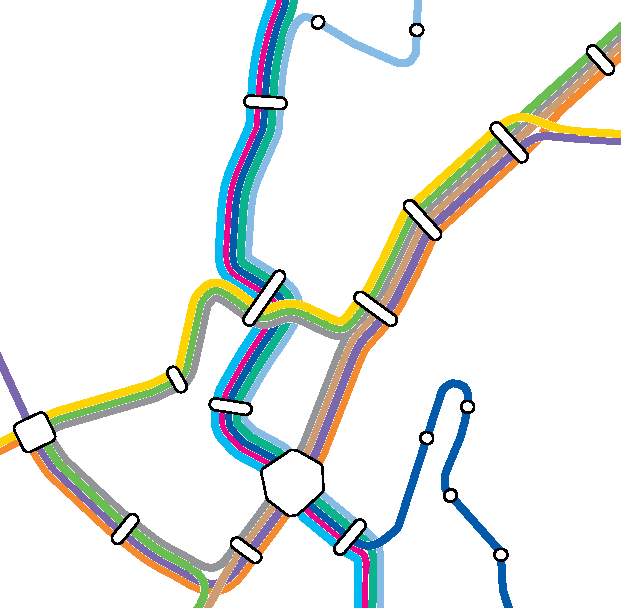
\includegraphics[trim={0cm 0 2.47cm 4.22cm},clip,width=0.44\textwidth]{render_examples/vvs_cropped.pdf}
	\caption{Left: transit graph of the light rail network in the center of Stuttgart, with traversing lines. Topological nodes are smaller. Right: transit map rendered from graph}
	\label{FIG:transitgraphvvs}
\end{figure}

Our goal is to render $T$ in a way that resembles a modern transit map (Figure~\ref{FIG:transitgraphvvs}). We want to globally optimize the ordering of lines in such a way that single lines can be easily traced through the network. This is usually formulated as the problem of minimizing the number of line crossings in the map and commonly called the Metro Line Crossing Minimization Problem (MLCM).

Classic MLCM assigns each edge $e=(u, v)$ two orderings $e_{u}$ and $e_{v}$ for $L(e)$, one at each node. Line crossings occur somewhere on $e$ if $e_{u} \neq e_{v}$ and crossings inside of nodes are prohibited. We propose an alternative model where only a single ordering is imposed on $L(e)$, meaning the ordering remains the same throughout $e$. This effectively disallows crossings on edges. Instead, we explicitely allow them in nodes (and favor crossings in topological nodes, see Section~\ref{SEC:crossing_placement}). We call this the MLTCM problem, the additional T stands for topological. In our opinion, this model better resembles the way transit maps are drawn manually. In real-world maps, crossings usually occur at positions where the network topology changes and crossings inside of stations are commonly. The model also greatly simplifies the rendering process (Section~\ref{SEC:rendering}), and \todo{other advantages.}

\todo{simple reduction to show that MLTCM is also NP-complete?}

%
\section{Network Topology Extraction}\label{SEC:topo}
%

Public transit data is usually given as a set of vehicle trips. A trip is an ordered list of served stations. The vehicle's geographical path may also be given. In recent years, the General Transit Feed Specification (GTFS) has become the dominant format for exchanging public transit schedules.

Because each trip is given explicitely, the transit graph induced by this data has many overlapping edges that may (partially) share the same geographical path. The network topology is usually lost.

Let $e_1, e_2$ be two edges in $T$ with their geometrical paths $\tau_{e_1}$ and $\tau_{e_2}$. We define a parametrization $\tau(\pi): [0,1] \mapsto \mathbb{R}^2$ which maps the progress $\pi$ to a point $p_d$ on $\tau$. For some distance threshold $\hat{d}$, we say $((\pi_1, \pi_2), ({\pi'}_1, {\pi'}_2))$ is a shared segment of $e_1$ and $e_2$ iff \[\forall (\pi, \pi'), \pi \in [d_1, {d'}_1], \pi' \in [d_2, {d'}_2] : \|\tau_{e_1}(\pi) - \tau_{e_2}(\pi')\| \leq d,\]

where $\|p - p'\|$ is the euclidean distance between $p$ and $p'$.

We restore the network topology and transform $T$ into a well-formed transit graph $T'$ by repeatedly collapsing shared segments between two edges $e_1, e_2$ into a single new edge $e_{12}$ until no more shared segments can be found. If for any of the edges the start of the shared segment $\pi$ lies not at the beginning of $\tau_e$, we split $e = (u, v)$ at $\pi$ into two edges $e'$ and $e''$ and introduce a new topological node $v'$ such that $e' = (u, v')$ and $e'' = (v', v)$ as well as $\tau_{e'}(1) = \tau_{e''}(0) = \tau_{e}(\pi)$. The same goes for the end point of a shared segment.

To find the shared segments between two paths $\tau$ and $\tau'$, we do a simple sweep over $\tau$ in $n$ steps of some $\Delta\pi$, measuring the distance $d$ between $\tau(i\cdot\Delta\pi)$ and $\tau'$ at each $i < n$ along the way. If $d \leq \hat{d}$, we start a new segment. If $d > \hat{d}$ and a segment is open, we close it. The algorithm can be made more robust against outliers by allowing $d$ to exceed $\hat{d}$ for a number of $n$ steps. It can be significantly sped up by indexing every linear segment of every path in a geometric index (for example, an R-Tree).

%
\section{Line Ordering Optimization}\label{SEC:ordering}
%

In this section, we describe an integer linear program (ILP) to solve MLTCM with $\mathcal{O}(|E|M^{2})$ variables and $\mathcal{O}(|E|M^{6})$ constraints.
Subsequently, we introduce an improved version with only $\mathcal{O}(|E|M^2)$ constraints and describe an extension to that ILP which solves MLTCM under the line separation constraint.

%
\subsection{Baseline ILP}\label{SEC:baseline}
%
For every edge $e \in E$, we define $|L(e)|^{2}$ decision variables $x_{elp} \in \{0,1\}$ where $e$ indicates the edge, $l \in L(e)$ the line, and $p=1, \cdots, |L(e)|$ the position/number of the line in the edge. We want to enforce $x_{elp}=1$ when line $l$ is assigned to edge number $p$ in the edge, and $0$ otherwise. This can be realized as follows:
\begin{equation*}
\forall l \in L(e): \sum_{p=1}^{L(e)} x_{elp}=1.
\end{equation*}
To assure that each position gets assigned exactly one line, we additionally need the constraints:
\begin{equation*}
	\forall p \in  \{1,\cdots,|L(e)|\} : \sum_{l \in L(e)} x_{elp} = 1.
\end{equation*}
\subsubsection{Avoiding crossings}\label{SEC:ac}
\begin{figure}
  \centering
	$\vcenter{\hbox{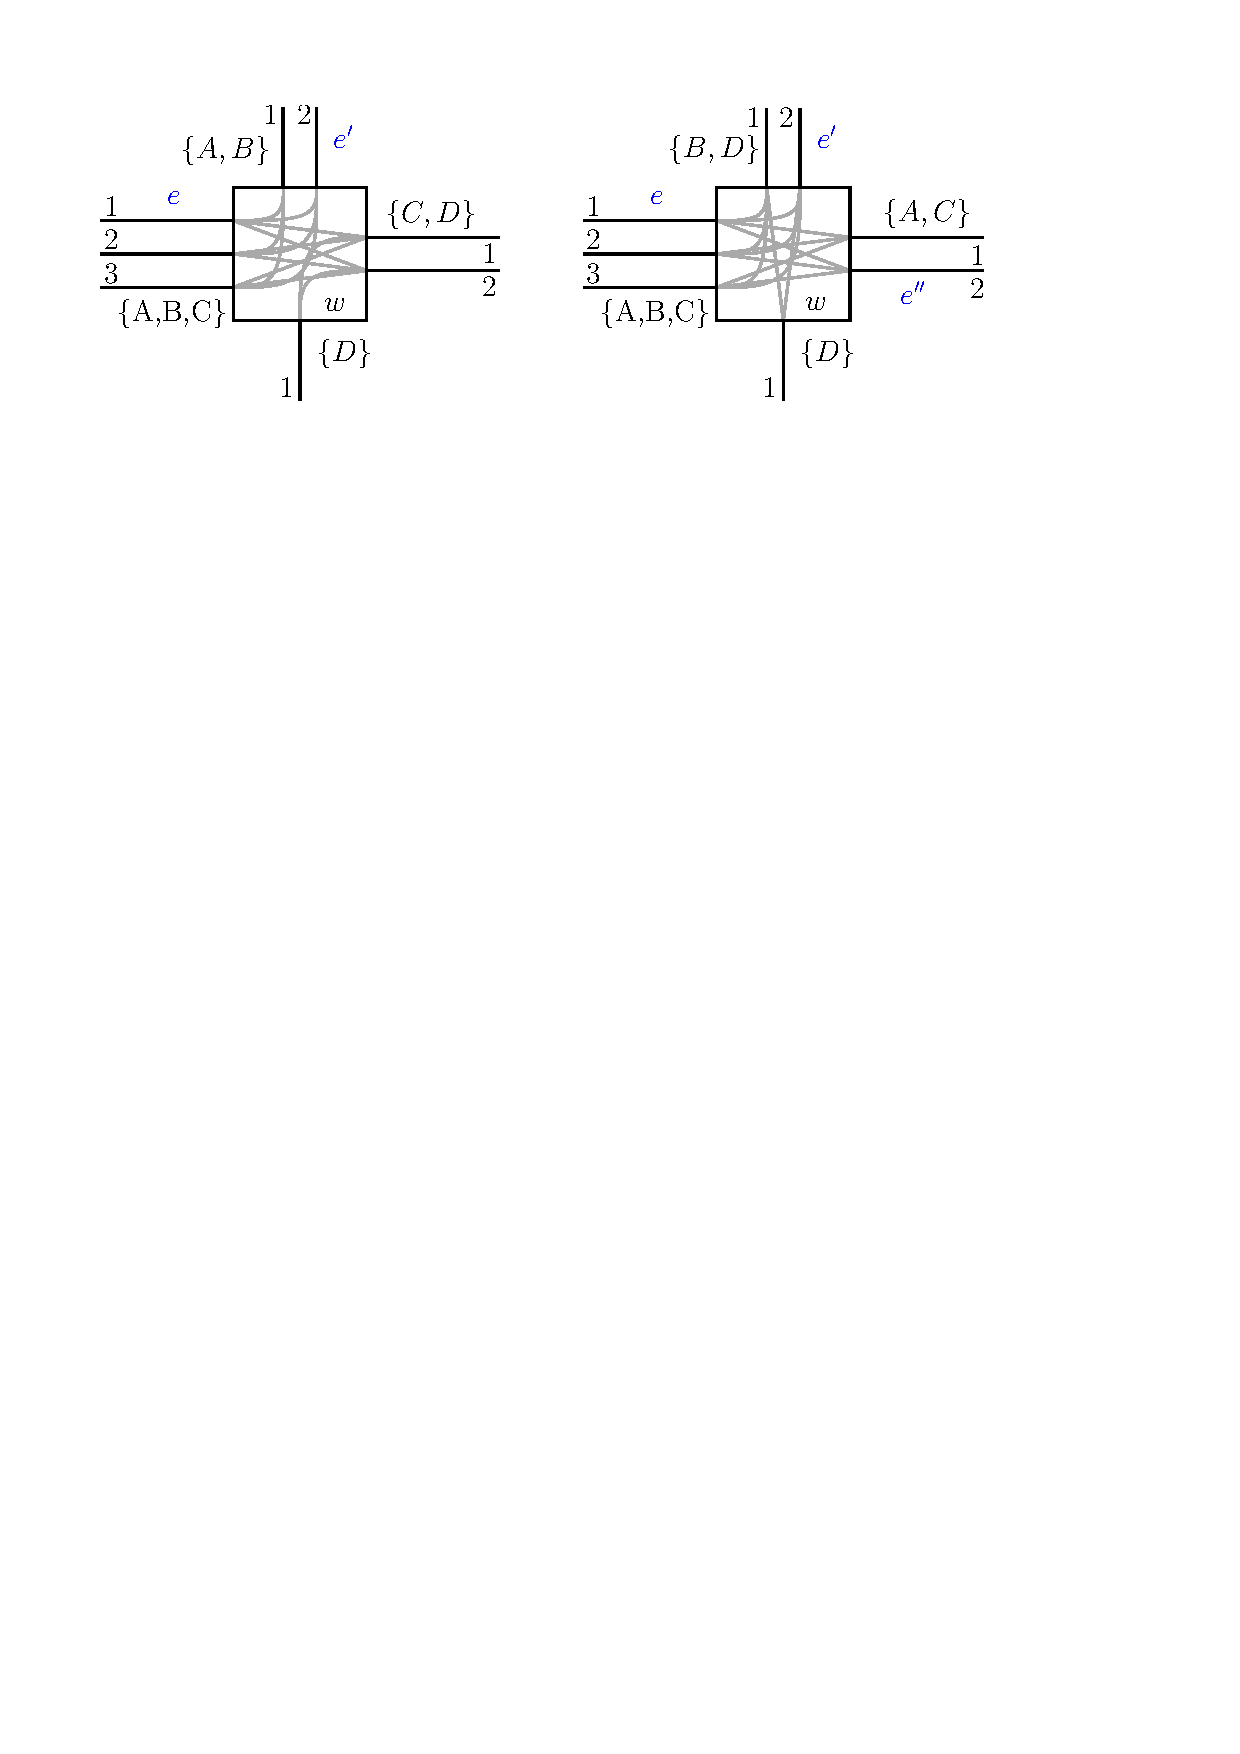
\includegraphics[width=0.6\textwidth]{crossing.pdf}}}$
	\caption{Example instance.}
	\label{FIG:crossings}
\end{figure}
Let $A, B$ be two lines belonging to an edge $e = \{v,w\}$ and both extend over $w$. We distinguish two cases: Either there is an adjacent edge $e'$ with $A,B \in L(e')$  or $A$ and $B$ continue in different edges, see Figure \ref{FIG:crossings}.

In the first case (left), $A, B$ induce a crossing if the position of $A$ is smaller than the position of $B$ in $L(e)$, so $p_e(A) < p_e(B)$, but vice versa in $L(e')$. We introduce the decision variable $x_{ee'AB} \in \{0,1\}$, which should be $1$ in case a crossing is induced and $0$ otherwise. To enforce this, we create one constraint per possible crossing. For example, a crossing would occur if we have $p_e(A)=1$ and $p_e(B)=2$ as well as $p_{e'}(A)=2$ and $p_{e'}(B) =1$. We encode this as follows:
\begin{equation*}
	x_{eA1} + x_{eB2} + x_{e'A2} + x_{e'B1} - x_{ee'AB} \leq 3.
\end{equation*}
In case the crossing occurs, the first four variables are all set to 1. Hence their sum is 4 and the only way to fulfill the $\leq 3$ constraint is to set $x_{ee'AB}$ to $1$. In the example given in Figure \ref{FIG:crossings}, six such constraints are necessary to account for all possible crossings of the lines $A$ and $B$ at node $w$.
The objective function of the ILP then minimizes the sum over all variables $x_{ee'AB}$.

In the second case (Figure \ref{FIG:crossings} right), $A$ and $B$ split into different edges $e', e''$. Then the actual positions of $A$ and $B$ in $e', e''$ do not matter, but the order of $e'$ and $e''$ itself. We introduce a split crossing decision variable $x_{ee'e''AB} \in \{0,1\}$ and constraints of the form
$\quad x_{eAi} + x_{eBj} - x_{ee'e''AB} \leq 1 \quad$
for all orders of $A$ and $B$ at $e$ with $i < j$ because in that case a crossing would occur. Likewise, $x_{ee'e''AB}$ is added to the objective function.

\subsubsection{ILP size}
Let $M = \max_{e \in E} |L(e)|$ be the maximum number of lines per edge. For mapping lines to positions at each edge we need $\leq |E|M^{2}$ variables and $\leq 2|E|M$ constraints. To minimize crossings, we have to consider $\leq M^{2}$ pairs of lines per edge, and introduce a decision variable for each such pair. That makes $\leq |E| M^{2}$ additional variables, which all appear in the objective function. Most constraints are introduced when two lines continue over a node in the same direction. In that case, we create $\leq \binom{M}{2}^{2} < M^{4}$ constraints per line pair per edge, so $\leq |E| M^{6}$ in total.
In summary, we have $\mathcal{O}(|E|M^{2})$ variables and $\mathcal{O}(|E|M^{6})$ constraints.

%
\subsection{Improved ILP Formulation}\label{SEC:improved}
%
The $\mathcal{O}(|E|M^{2})$ variables in the baseline ILP seem to be reasonable, as indeed $\Omega(|E|M^{2})$ crossings could occur. But the $\mathcal{O}(|E|M^{6})$ constraints are due to enumerating all possible position inversions explicitly. If we could check the statement \emph{position of A on $e$ is smaller than the position of B} efficiently, the number of constraints could be reduced. To have such an oracle, we first modify the line-position assignment constraints.

\subsubsection{Alternative line-position assignment}
Instead of a decision variable which encodes the exact position of a line in an edge as before, we know use $x_{el\leq p} \in \{0,1\}$ which is $1$ if the position of $l$ in $e$ is $\leq p$ and $0$ otherwise. To enforce a unique position, we use the constraints:
\begin{align}
	\forall l \in L(e)~ \forall p \in \{1, \cdots, |L(e)|-1\}: \quad x_{el\leq p} \leq x_{el\leq p+1}. \label{EQ:up_constr}
\end{align}
This ensures that the sequence can only switch from $0$ to $1$, and this exactly once. To make sure that at some point a $1$ appears and that each position is occupied by exactly one line, we additionally introduce the following constraints:
\begin{align}
	\forall p \in \{1, \cdots, |L(e)|\}: \sum_{l \in L(e)} x_{el\leq p} = p. \label{EQ:01_constr}
\end{align}
So exactly for  one line $x_{e.\leq 1} =1$ is true, for two lines $x_{e.\leq 2} = 1$ (of which one has to fulfill $x_{e.\leq 1} =1$) and so on.

\subsubsection{Crossing Oracle}
We reconsider the example from \ref{SEC:ac}, left. Before, we enumerated all possible positions which induce a crossing for $A, B$ at the transition from $e$ to $e'$. But it would be sufficient to have variables which tell us whether the position of $A$ is smaller than the position of $B$ in $e$, and the same for $e'$, and then compare those variables. For a line pair $(A,B)$ on edge $e$ we call the respective variables $x_{eA>B}, x_{eA<B} \in \{0, 1\}$. %Since we introduce these variables for each line pair in $e$, $x_{eA<B}$ will re-appear as $x_{eB>A}$, so we only need $x_{eA>B}$.
To get the desired value assignments, we add the following constraints:
\begin{gather}
	\sum_{p=1}^{|L(e)|} x_{eA\leq p} - \sum_{p} x_{eB\leq p} + x_{eA>B} M \geq 0 \\
	x_{eA>B} + x_{eA<B}=1.
\end{gather}
The equality constraints make sure that not both $x_{eA>B}$ and $x_{eB>A}$ can be $1$. If the position of $A$ is smaller than the position of $B$, then more of the variables corresponding to $A$ are $1$, and hence the sum for $A$ is higher. So if we subtract the sum for $B$ from the sum for $A$ and the result is $\geq 0$, we know the position of $A$ is  smaller and $x_{eA>B}$ can be $0$. Otherwise, the difference is negative, and we need to set $x_{eA>B}$ to $1$ to fulfill the inequality. It is then indeed fulfilled for sure as the position gap can never exceed the number of lines per edge.

To finally decide if there is a crossing, we would again like to have a decision variable $x_{ee'AB} \in \{0,1\}$ which is $1$ in case of a crossing and $0$ otherwise -- and minimize the sum of all such variables in the objective function.
The constraint
\begin{gather}
	abs(x_{eA<B}-x_{e'A<B}) - x_{ee'AB} \leq 0
\end{gather}
realizes this, as either $x_{eA<B} = x_{e'A<B}$ (both $0$ or both $1$) and then $x_{ee'AB}$ can be $0$, or they are unequal and hence the absolute value of their difference is $1$, enforcing $x_{e'AB}=1$. As absolute value computation can not be part of an ILP we use the following equivalent standard replacement:
\begin{align}
	x_{eA<B} - x_{e'A<B} - x_{ee'AB} &\leq 0 \label{EQ:abs_upper}\\
	-x_{eA<B} + x_{e'A<B} - x_{ee'AB} &\leq 0. \label{EQ:abs_lower}
\end{align}
%If the values are equal, nothing changes in the argumentation. If the values are unequal, either (\ref{EQ:abs_upper}) or (\ref{EQ:abs_lower})  will produce a $1$ as the sum of the first two terms, enforcing $x_{ee'AB}=1$ as desired.

\subsubsection{Complexity of the improved ILP}
For the line-position assignment, we need at most $\leq |E|M^{2}$ variables and constraints just like before. For counting the  crossings, we need per pair of lines per edge only a constant number of new variables and constraints as shown above, hence $\mathcal{O}(|E|M^{2})$ in total.

\subsection{Placement of Inevitable Crossings}\label{SEC:crossing_placement}

Inevitable crossings are enforced by the network's topology. In the ILPs described above, the placement of these crossings largely depends on the solver's strategy.

We want to favor crossing placements in topological nodes ($v_\sigma = 0$). We also found that favoring nodes that have a higher count of incident edges as a location for crossings yields maps that appear more well-arranged.
Since all of these criteria are invariant to the orderings imposed on the $L(E)$, we can control the placements by simply introducing a weighting factor $k_{ee'}$ which is added with each $x_{ee'll'}$ to the objective function.
The value of $k_{ee'}$ depends on the node where $e$ and $e'$ meet and is set like described above.

\subsection{Preventing Line Partner Separation}\label{SEC:separation}
So far, we only optimized the number of line crossings. However, consider the example given in Figure~\ref{FIG:linesplitting}, where the ordering with more crossings looks better.
\begin{figure}
\centering
\begin{minipage}{.48\textwidth}
  \centering
	
\includegraphics[angle=270,origin=c,width=.3\textwidth]{render_examples/splitting_example_nonopt.pdf}\hspace{10pt}
	
\includegraphics[angle=270,origin=c,width=.3\textwidth]{render_examples/splitting_example.pdf}
	\caption{Crossings are minimized in the left example (1), but the right one better indicates line pairings.}
	\label{FIG:linesplitting}
\end{minipage}%
\hfill
\begin{minipage}{.48\textwidth}
  \centering
	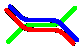
\includegraphics[angle=90,origin=c,width=.3\textwidth]{render_examples/splitting_example2_nonopt.pdf}\hspace{10pt}
	
\includegraphics[angle=90,origin=c,width=.3\textwidth]{render_examples/splitting_example2.pdf}
	\caption{Both orderings have the same number of crossings (2), but in the right one the
crossing is done in one pass.}
	\label{FIG:linesplitting2}
\end{minipage}
\end{figure}
A similar problem can be seen in Figure~\ref{FIG:linesplitting2}. In both cases, we can adress the problem by punishing the separation of lines. For two adjacent edges $e$ and $e'$ and a line pair $(A, B$) that continues from $e$ to $e'$, if $A$ and $B$ were placed next to each other in $e$ (were partners in $e$) but not anymore in $e'$, we want to add some penalty to the objective function. For this, we introduce a variable $x_{eA\|B} \in \{0, 1\}$. Let $p_{eA}$ be the position of $A$ in $e$ and $p_{eB}$ the position of $B$ in $e$. We want $e_{sA\|B}$ to be $1$ if $\left|p_{eA} - p_{eB}\right| = 0$ (if they occur next to each other) and $1$ otherwise. To get the desired assignments, we add the following constraints per line pair in $e$:
\begin{align}
	\sum_{p=1}^{|L(e)|} x_{eA\leq p} - \sum_{p} x_{eB\leq p} - x_{eA\|B} M &\leq 1 \label{EQ:sep_cstr_1} \\
	\sum_{p=1}^{|L(e)|} x_{eB\leq p} - \sum_{p} x_{eA\leq p} - x_{eA\|B} M &\leq 1. \label{EQ:sep_cstr_2}
\end{align}
If $p_{eA} = p_{eB}$, then the difference of the sums in both constraints is 0. If $|p_{eA} - p_{eB}| = 1$, then the sum difference in both constraints is $\leq 1$. If $|p_{eA} - p_{eB}| > 1$, then either (\ref{EQ:sep_cstr_1}) or (\ref{EQ:sep_cstr_2}) enforce $x_{eA\|B} = 1$. To prevent the trivial solution where $x_{A\|B}$ is 1 for all line pairs, we introduce the following additional constraint per edge:
\begin{align*}
	\sum_{l \in L(e)}\sum_{l' \in L(e)} x_{el\|l'} \leq |L(e)|^2 - 3|L(e)| - 2
\end{align*}
as indeed the maximal number of line pairs in $e$ (excluding lines paired with themselves) is $|L(e)|^2 - |L(e)|$ and the number of $x_{el\|l'}$ in $e$ that are 0 is exactly $2|L(e)| - 2$ (each line is next to its two neighbors, but the first and last line only have 1 neighbor). A fixed constraint is not necessary here, however, because the lower bound is already provided by the line pair constraints (\ref{EQ:sep_cstr_1}) and (\ref{EQ:sep_cstr_2}).

Like in Section~\ref{SEC:improved}, we introduce a decision variable $x_{ee'A\|B} \in \{0, 1\}$ that should be $1$ if $A$ and $B$ are splitted between $e$ and $e'$ and $0$ otherwise:
\begin{align*}
	x_{eA\|B} - x_{e'A\|B} - x_{ee'A\|B} &\leq 0 \\
	-x_{eA\|B} + x_{e'A\|B} - x_{ee'A\|B} &\leq 0.
\end{align*}
$x_{ee'A\|B}$ is added to the objective function. If $|L(e)| = |L(e')| = 2$, a line separation penalty is not needed for $A$ and $B$ because they will always be next to each other. If only $|L(e)| = 2$, we can add $x_{e'A\|B}$ to the objective function directly (and likewise if only $|L(e')|=2$).

\todo{Mention the special case of the MLCM-P periphery constraint the above constraints handle out-of-the-box}

\subsubsection{Complexity}
We add $1$ additional constraint per edge in $e$ and a constant number of additional constraints and variables per line pair to the ILP, so the number of variables and constraints is still in $\mathcal{O}(|E|M^2)$.

%
\subsection{Core problem graph}\label{SEC:coreprobgraph}
%
An inevitable crossing (or separation) between two lines $j$ and $k$ can only occur if there is at least one node $v_{jk}$ with one of the following properties:
\begin{enumerate}
\item $v_{jk}$ is adjacent to $e : j \not\in L(e) \land k \in L(e')$ and $e' : j \in L(e') \land k \not\in L(e)$. \label{EQ:liaisonnode}
\item $|{e \in adj(v_{jk}) : j \in L(e) \land i \in L(e)}| > 2$. \label{EQ:tnode}
\end{enumerate}
\begin{proof} If no such node exists, then it holds for all $v \in V$ that $j$ and $k$ either both travel through $v$ on the same two edges or they don't travel together through $v$ at all. In the latter case, no crossing (or separation) can occur and we can thus disregard it, which leaves us only with the former case. But if $j$ and $k$ travel through all nodes together on the same two edges, then the relative order of $j$ and $k$ does not matter anymore - we can just combine $j$ and $k$ into a new line $i$ and assign $j$ and $k$ an arbitrary global ordering.
\end{proof}

We call nodes that comply to (\ref{EQ:liaisonnode}) for a line pair $A = \{j, k\}$ a liaison node for $j$ and $k$ and nodes that comply to (\ref{EQ:tnode})  a T-node for $j$ and $k$. Additionally, we call a node that is a liaison and/or T-node for at least one line pair an intersection node and a node in which one or more lines end a terminus node.

Using the above, we can simplify the input graph prior to optimization with the following steps:
\begin{enumerate}
\item collapse lines that always occur together into a single new line
\item delete each node with degree 2 (adjacent to edges $e = (u, v)$ and $e' = (v, w)$) and $L(e) = L(e')$ and combine $e$ and $e'$ into a single new edge $ee' = (u, w)$ with $L(ee') = L(e) = L(e')$ . Note that such a node can never be a terminus node or an intersection node.
\end{enumerate}
Since we never delete an intersection node, these operations will not affect the optimality of the found solution. In practice, they will move line crossings to liaison nodes or T-nodes. This has a similar effect as the heuristic described in Section~\ref{SEC:crossing_placement}.

This core problem graph can be further prepared for optimiziation by splitting it into ordering-relevant connected components using the following rules:
\begin{enumerate}
	\item cut each edge $e = (u, v)$ with $|L(e)| = 1$ into two edges $e' = (u, v')$ and $e'' = (v'', v)$. Note that $v'$ and $v''$ are not connected.
	\item replace each edge $e = (u, v)$ where $v$ is a terminus node for each $l \in L(e)$ with an edge $e' = (u, v'$ where $v'$ is only connected to $e'$. Delete $e$ from the adjaceny list of $v$.
	\item remove each edge $e = (u, v)$ where $u$ and $v$ are termini for all $l \in L(e)$
\end{enumerate}
The line-ordering optimization can now be run independently on each connected component of the core problem graph.
\begin{figure}[h]
\centering
	\includestandalone[width=5cm]{tikz/transitgraph_optim}
	\hspace{0.6cm}
	\includestandalone[width=4.4cm]{tikz/coreoptimgraph}
	\caption{Left: transit graph $G$ with lines $a, b, c, d, e, f$, Right: core optimization graph with highlighted ordering-relevant connected components with more than 1 node; $ab$ was collapsed into $x$.}
\end{figure}

%
\section{Rendering}\label{SEC:rendering}
%
\todo{short explanation of parallel line rendering, node front expansion for non-station nodes, explain bezier curve and explain degeneration to circle arc}

%
\section{Evaluation}
%

To test our edge ordering optimization method, we ran it against the public transit schedules of several cities around the world (Table~\ref{TBL:datasets}). Each dataset was first transformed into a well-formed transit graph using the method described in Section~\ref{SEC:topo}. After that, an edge ordering optimization run was started for each city.

%
\subsection{Optimization Results}
%

We evaluated the size of the resulting ILP using the baseline approach from Section~\ref{SEC:baseline} as well as the improved version from Section~\ref{SEC:improved}. We also compared the ILPs resulting from the reduced core optimization graph against those generated from the raw transit graph. Each ILP was then given to the GNU Linear Programming Kit (glpk) and the COIN-OR CBC (coin) solver. For the improved approach, we tested each dataset with or without the line separation penalty described in Section~\ref{SEC:separation}.
\begin{table}
	\centering
	\footnotesize
	\begin{tabular*}{1\textwidth}{@{\extracolsep{\fill}} l r r r r r r r r r r}
							& \multicolumn{5}{ c }{\scriptsize Transit graph} & \multicolumn{5}{ c }{\scriptsize Core optimization graph} \\[-1.4ex]
							& \multicolumn{5}{ c }{\scriptsize \downbracefill} & \multicolumn{5}{ c }{\scriptsize \downbracefill} \\
							& $|V_{\sigma=1}|$ & $|V_{\sigma=0}|$ & $|E|$ & $|L|$ & ${|L(e)|}_{\text{max}}$ & $|V|$ & $|E|$ & $|L|$ & ${|L(e)|}_{\text{max}}$ \\[-2.5ex] \\\hline \\[-2ex]

		Freiburg Trams		& 100	& 45	 & 5	& 120	& 65	& 65	& 40	& 5		& 4		\\
		Boston				& 100	& 39	 & 8	& 120	& 12	& 65	& 40	& 5		& 4		\\
		Chicago				& 54	& 15	 & 3	& 120	& 2		& 65	& 40	& 5		& 4		\\
		Dallas				& 100	& 457	 & 3	& 120	& 66	& 65	& 40	& 5		& 4		\\
		San Francisco		& 100	& 45	 & 5	& 120	& 3		& 65	& 40	& 5		& 4		\\
		NYC Subway			& 2585	& 545	 & 17	& 120	& 8		& 65	& 40	& 5		& 4		\\
		Manhattan Busses	& 7880	& 145	 & 5	& 120	& 43	& 65	& 40	& 5		& 4		\\
		\noalign{\vspace{.8mm}}\hline\noalign{\vspace{1.5mm}}
	\end{tabular*}
	\caption[]{Testing datasets and their transit graph after spatial topology extraction \todo{enter real data here}\label{TBL:datasets}}
\end{table}

\begin{table}
	\centering
	\footnotesize
	\begin{tabular*}{1\textwidth}{@{\extracolsep{\fill}} l r r r r r r r r r r}
							& \multicolumn{4}{ c }{\scriptsize with graph reduction} & \multicolumn{4}{ c }{\scriptsize without graph reduction} \\[-1.4ex]
							& \multicolumn{4}{ c }{\scriptsize \downbracefill} & \multicolumn{4}{ c }{\scriptsize \downbracefill} \\
							& rows & cols & $t_\text{glpk}$ & $t_\text{coin}$  & rows & cols & $t_\text{glpk}$ & $t_\text{coin}$ & cross. & sep. \\[-2.5ex] \\\hline \\[-2ex]

		Freiburg Trams		& 100	& 45	 & 5	& 120	& 65	& 40	& 5		& 4		& 6		& 7		\\
		\hspace{2mm}\scriptsize
		(with sep. penalty)	& 100	& 45	 & 5	& 120	& 65	& 40	& 5		& 4		& 6		& 7		\\
		Boston				& 100	& 39	 & 8	& 120	& 12	& 40	& 5		& 4		& 6		& 7		\\
							& 100	& 45	 & 5	& 120	& 65	& 40	& 5		& 4		& 6		& 7		\\
		Chicago				& 54	& 15	 & 3	& 120	& 2		& 40	& 5		& 4		& 6		& 7		\\
							& 100	& 45	 & 5	& 120	& 65	& 40	& 5		& 4		& 6		& 7		\\
		Dallas				& 100	& 457	 & 3	& 120	& 66	& 40	& 5		& 4		& 6		& 7		\\
							& 100	& 45	 & 5	& 120	& 65	& 40	& 5		& 4		& 6		& 7		\\
		San Francisco		& 100	& 45	 & 5	& 120	& 3		& 40	& 5		& 4		& 6		& 7		\\
							& 100	& 45	 & 5	& 120	& 65	& 40	& 5		& 4		& 6		& 7		\\
		NYC Subway			& 2585	& 545	 & 17	& 120	& 8		& 40	& 5		& 4		& 6		& 7		\\
							& 100	& 45	 & 5	& 120	& 65	& 40	& 5		& 4		& 6		& 7		\\
		Manhattan Busses	& 7880	& 145	 & 5	& 120	& 43	& 40	& 5		& 4		& 6		& 7		\\
							& 100	& 45	 & 5	& 120	& 65	& 40	& 5		& 4		& 6		& 7		\\
		\noalign{\vspace{.8mm}}\hline\noalign{\vspace{1.5mm}}
	\end{tabular*}
	\caption[]{ILPs generated with improved approach, with or without graph reduction and separation penalty. Solving times with glpk or COIN \todo{enter real data here}\label{TBL:evalres}}
\end{table}

%
\subsection{Aesthetical Evaluation}
%

%
\section{Further work}
%

\todo{mention that our model forces a line crossing in a station if a topology change happens inside of this station. in this case, it may be useful to add "fake" topology nodes outside of the station}

\todo{mention thorough aesthetical evaluation via crowdsourcing}


\bibliographystyle{plain}
\bibliography{tm.bib}

\end{document}
